\chapter{Path Planning} \label{ch:pp}
The goal of the planner introduced is to assist in the discovery of a field's features with a tunable level of speed and confidence of prediction. The user of such a system could choose to scan more area if fuel is not of high concern. Likewise, if the field is very large, or several fields need to be scanned in a limited amount of time, a quicker scan with a lower degree of prediction certainty can be performed.

\section{Uncertainty Loss Function} \label{sec:lossfunc}
In Section \ref{sec:fielduncert}, a criteria for overall field uncertainty was introduced. Given a set of previously sampled points, $S$, and a new set of samples, $T$, a new field uncertainty can be calculated via $\Sigma_{\text{var}}(\hat{Z}(S + T))$, where $S + T$ is the union of the the two sets $S$ and $T$. Given a new set of samples, $T$, the loss in a target field's prediction uncertainty, $L(T)$, is a metric that should be maximized by a path planner aiming to improve prediction quality for exploration purposes.

\begin{equation}
	L(T) = (\Sigma_{\text{var}}(\hat{Z}(S+T)) - \Sigma_{\text{var}}(\hat{Z}(S)))
	\label{eq:lossfunc}
\end{equation}

The optimal path, $O$, subject to a limited scanning time constraint, is the path that simultaneously maximizes $L(O)$, and minimizes the length of of the path taken (using the assumption of a constant linear velocity from Section \ref{sec:vehicledynamics}), $l(S + O)$.

\begin{equation}
	O = \argmax_T\ \beta L(T) - (1-\beta)l(S + T)
\end{equation}

Where $\beta \in [0,1]$ is a real number which puts more emphasis on exploration time over prediction quality. It is important to note that as more samples are taken, the overall field prediction variances change. It would be in the benefit of a path planner to batch process a set of points after meeting a predetermined waypoint, or after a threshold number of samples. 

Given an endpoint in a single trajectory, in the limit, recalculating $O$ at every sample would optimally shape the trajectory of the exploration vehicle. With no endpoint selected, the exploration vehicle could be found in a repeating state due to being stuck in a global minimum in the variance field. In an effort to avoid the sticking minimum problem, the path planners introduced will be endpoint oriented (where the endpoint of any trajectory is predetermined), and the goal of each path taken is to make it to the endpoint. Furthermore, a new path will only be calculated as a batch process after sampling a trajectory. This is done in an attempt to reduce computation time as the Kriging predictions and variance calculations become more expensive as more samples are taken.

\section{Finding Points of Highest Uncertainty} \label{sec:highestvars}
Points on a target field with high prediction variances are points on a field that can be sampled first, in turn maximizing $L$ in Equation \ref{eq:lossfunc}. After sampling an initial set of points, and then running a Kriging prediction on all points on a target, the variance of prediction of all points can be calculated.

The motivation of the path finders introduced are to minimize the average uncertainty of a target field, by to sampling the points representing the highest prediction variance. A set of points where the highest uncertainties lay are found on the field using a simple search.

Let $S_k$ be a singleton set containing the point of highest variance on the $k^{th}$ iteration of the target field prediction variances, represented as the set $\text{var}\{\hat{Z}_k\}$, where $\text{var}\{\hat{Z}\} : \mathbb{R}^2 \to \mathbb{R}^+$.

\begin{equation}
	S_{k} = \argmax_{\vect{s}} \ \text{var}\{\hat{Z}_{k}(\vect{s})\}
	\label{eq:highestvar}
\end{equation}

The cardinality of the set $S_k$ can be greater than one if there exist multiple instances of the same value of variance in the target field prediction variances. For the sake of simplicity, only the singleton case will be considered.

Let $\text{var}\{\hat{Z}_{k+1}\}$ be the set of points, not including the point of highest variance found in the $k^{th}$ iteration of the set configuration (Equation \ref{eq:highestvar}), on a target field prediction.

\begin{equation}
	\text{var}\{\hat{Z}_{k+1}(\vect{s})\} = \text{var}\{\hat{Z}_k(\vect{s})\} - S_k \\
	\label{eq:nextmaxvarsset}
\end{equation}

Let $S_{v}$ be the set of the $N$ points of highest uncertainty on the target field prediction variances, $\text{var}\{\hat{Z}\}$.

\begin{equation}
	\label{eq:highestvarsunion}
	S_{v} = \bigcup_{k = 1}^{N} S_k = \bigcup_{k = 1}^{N} \text{var}\{\hat{Z}_k(\vect{s})\} - \text{var}\{\hat{Z}_{k+1}(\vect{s})\}
\end{equation}

\section{Next Highest Variance (NHV) Trajectory Finding} \label{sec:nhvtrajfind}
Sampling the location of the next highest variance (NHV) is the simplest and most naive approach to path planning using the Kriging method. By finding the highest variance in the field using Equation \ref{eq:highestvar}, and setting $N=1$ in \ref{eq:highestvarsunion}, the next endpoint is found. Setting the destination, $\vect{s}_d$, to the found waypoint in $S_{v}$, and knowing the current location, $\vect{s}_{c}$, a set of waypoints that establish the route between the start and finish points can be defined as $T = \Big\{[x_{1}\ y_{1}\ \theta_{1}]^T,\ [x_{2}\ y_{2}\ \theta_{2}]^T, \dots [x_{{i_f}}\ y_{{i_f}}\ \theta_{{i_f}}]^T \Big\}$, $i_f = \Big\lceil \frac{\|\vect{s}_c - \vect{s}_d\|_2}{\alpha} \Big\rceil$, where, $\alpha \in \mathbb{R}^{+}$, is a scaling variable representing the step size between waypoints, $x$ and $y$ are field coordinates, and $\theta$ is the heading angle of the vehicle. 

\begin{equation}
	\label{eq:nhvtrajectory}
	T_{{i + 1}} = T_{i} +
	\begin{bmatrix}
		\alpha \cos \theta_{i} \\
		\alpha \sin \theta_{i} \\
		\text{atan2}(s_{d_y} - T_{{{i+1}_y}}, s_{d_x} - T_{{{i+1}_x}}))
	\end{bmatrix}
\end{equation}

The initial point, $T_{1}$, is defined explicitly.

\begin{equation}
	T_{1} = \begin{bmatrix}
		s_{c_x} \\
		s_{c_y} \\
		\text{arctan2}(s_{d_y} - s_{c_y}, s_{d_x} - s_{c_x})
	\end{bmatrix}
\end{equation}

\subsection{NHV Path Planning Algorithm} \label{sec:nvh_pp_alg}
The exploration algorithm initializes by directing the vehicle to sweep across the forward diagonal of the target field to collect an initial set of samples. An initial variogram is fit, and a Kriging prediction of the field is then made. The variances of all points on the target field are then calculated. The point with the highest prediction variance is found (Section \ref{sec:highestvars}). The trajectory, $T$, is then calculated (Section \ref{sec:nhvtrajfind}), and set as the path to take. Once the vehicle completes the last path chosen, the field values and variances are predicted and calculated again. A new path is chosen in the same fashion. The algorithm terminates when it can no longer choose a path that can be accomplished with the amount of fuel that remains within the exploration vehicle. Another case of planner termination occurs When the average prediction variance of the field is zero, which ideally occurs when all locations have been sampled. See Figure \ref{fig:nhv_pp} for a short 1\% capped version of the algorithm.

\begin{figure}[hb!]
	\centering
	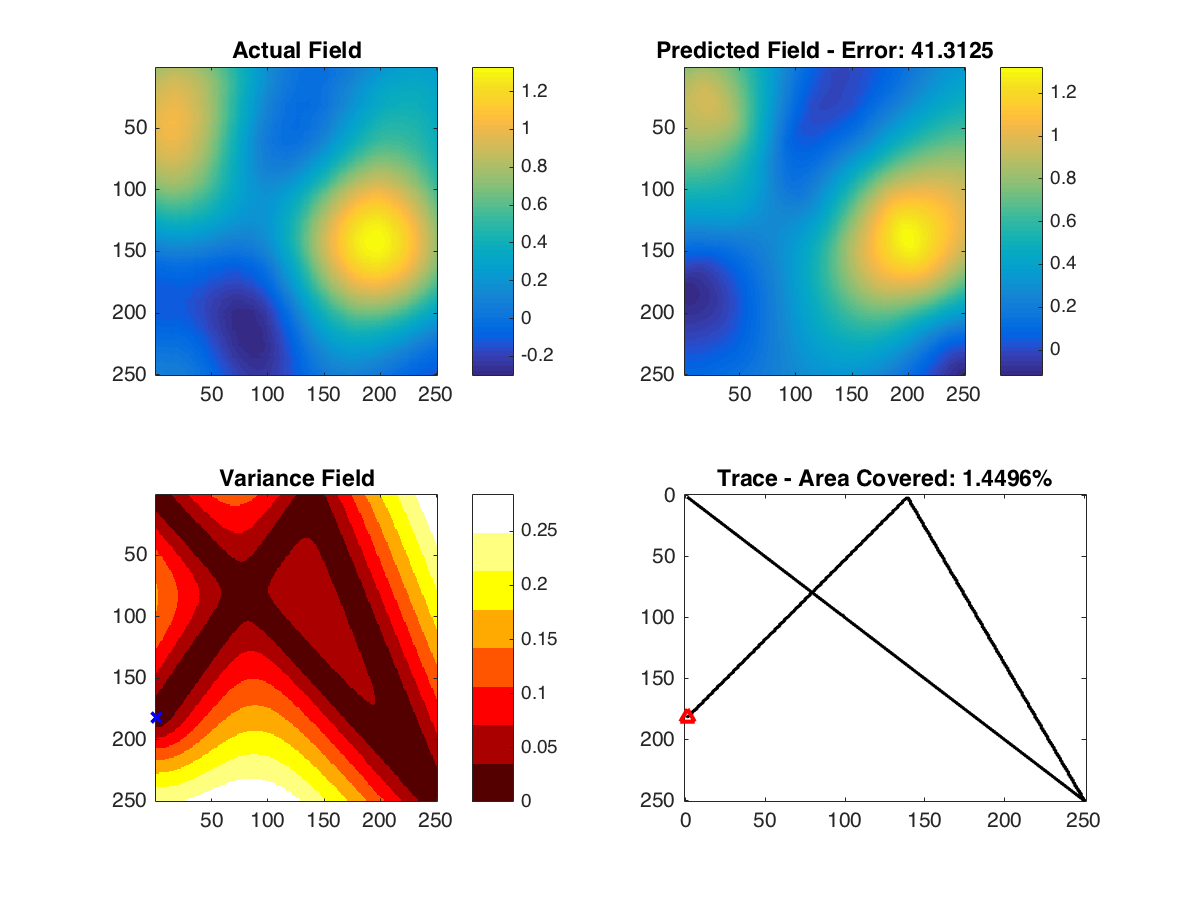
\includegraphics[width=0.95\linewidth]{figures/nhv_4panel.png}
    \captionsetup{skip=0.20\baselineskip,size=footnotesize}
	\caption{The Next Highest Variance (NHV) algorithm (Section \ref{sec:nvh_pp_alg} terminated after two iterations of the algorithm. The actual field that is being explored is shown in the upper left. The current prediction of the actual field is shown in the upper right. The variance of the current prediction of the field is shown in the lower left. The trace of the exploration vehicle's path taken to the point of termination (in red) is shown in the lower right panel. All distance units are in meters.}
	\label{fig:nhv_pp}
\end{figure}

\subsection{Inefficiency in NHV}
The NHV algorithm does not account for repeating paths, or avoiding re-sampling points. The only knowledge used is a single criteria of variance. Although the ground covered by the algorithm may be sufficient for the most exploration cases, a path planner that considers the cost of trajectories would likely yield better results.

\section{Monte Carlo Based Trajectory Finding}
A path planner designed for autonomous field exploration using a Monte Carlo path selection technique will be introduced. By first selecting a set of locations with the highest uncertainty in current prediction, the path planner will find a suitable path that will in turn minimize the average variance of the target field predictions. The problem can be stated as a sensor placement problem, where a suitable placement of sensors is found via a Monte Carlo simulation of the environment, and a minimization of the Kriging prediction variances \cite{kriging:sensorplacement}. Using Monte Carlo for trajectory finding for obstacle avoidance has been attempted \cite{janson:mcmp}, but not for exploration purposes.

In the case of the path planner, because the exploration vehicle is dynamic, the sensors can be thought of as being placed along the trajectory of the vehicle (assuming reasonable ergodicity of the target field). The Monte Carlo approach to path finding via the Kriging Method introduced will first find the points of highest prediction uncertainty on the target field, and then generate a finite set of random trajectories along the originally found trajectories. The trajectory that is predicted to reduce overall field uncertainty will be chosen as the path the vehicle will take.

\subsection{Finding Monte Carlo Trajectory Sets} \label{sec:mctrajsets}
After a suitable set of destinations are selected from the set of points containing the $N^{th}$ coordinates of highest uncertainty, $S_{v}$, trajectories to each point are calculated. The trajectories calculated can be both deterministic or variably non-deterministic walks from the current location of the exploration vehicle, to the final location.

For a given destination, $\vect{s}_d$ in $S_{v}$, and the current location of the vehicle, $\vect{s}_{c}$, a set of waypoints that establish the route between the start and finish points can be defined as $T_k = \Big\{[x_{k_1}\ y_{k_1}\ \theta_{k_1}]^T,\ [x_{k_2}\ y_{k_2}\ \theta_{k_2}]^T, \dots [x_{k_{i_f}}\ y_{k_{i_f}}\ \theta_{k_{i_f}}]^T \Big\}$, $i_f = \Big\lceil \frac{\|\vect{s}_c - \vect{s}_d\|_2}{\alpha} \Big\rceil$, where, $\alpha \in \mathbb{R}^{+}$, is a scaling variable representing the step size between waypoints, $x$ and $y$ are field coordinates, and $\theta$ is the heading angle of the vehicle. 

\begin{equation}
	T_{k_{i + 1}} = T_{k_i} +
	\begin{bmatrix}
		\alpha \cos \theta_{k_i} \\
		\alpha \sin \theta_{k_i} \\
		\text{atan2}(s_{d_y} - T_{k_{{i+1}_y}}, s_{d_x} - T_{k_{{i+1}_x}}))
	\end{bmatrix} + \begin{bmatrix} 
		\vect{w}_{k_{i+1}} \\
		0
	\end{bmatrix}
\end{equation}

Where $\vect{w}_k \in \mathbb{R}^2$ is a zero-mean Wiener Process with a tunable variance. Multiple Brownian walks from the current position to a given destination can be calculated to increase the pool of possible paths. For a zero variance Wiener process ($\text{var}\{\vect{w}\}=0$), the walk defined is deterministic, and equal to finding a set of N-NHV trajectories (Section \ref{sec:nnhv}. The \textit{cord} of the walk is the line the connects the initial position to the destination position. The cord acts as the expected value in the distribution of trajectories calculated. The initial point, $T_{k_1}$, and the final point, $T_{k_f}$, are defined explicitly.

\begin{equation}
	T_{k_1} = \begin{bmatrix}
		s_{c_x} \\
		s_{c_y} \\
		\text{arctan2}(s_{d_y} - s_{c_y}, s_{d_x} - s_{c_x})
	\end{bmatrix},\ 
	T_{k_f} = \begin{bmatrix}
		s_{d_x} \\
		s_{d_y} \\
		\theta_{f-1}
	\end{bmatrix}
\end{equation}

\begin{figure}[h!]
	\centering
	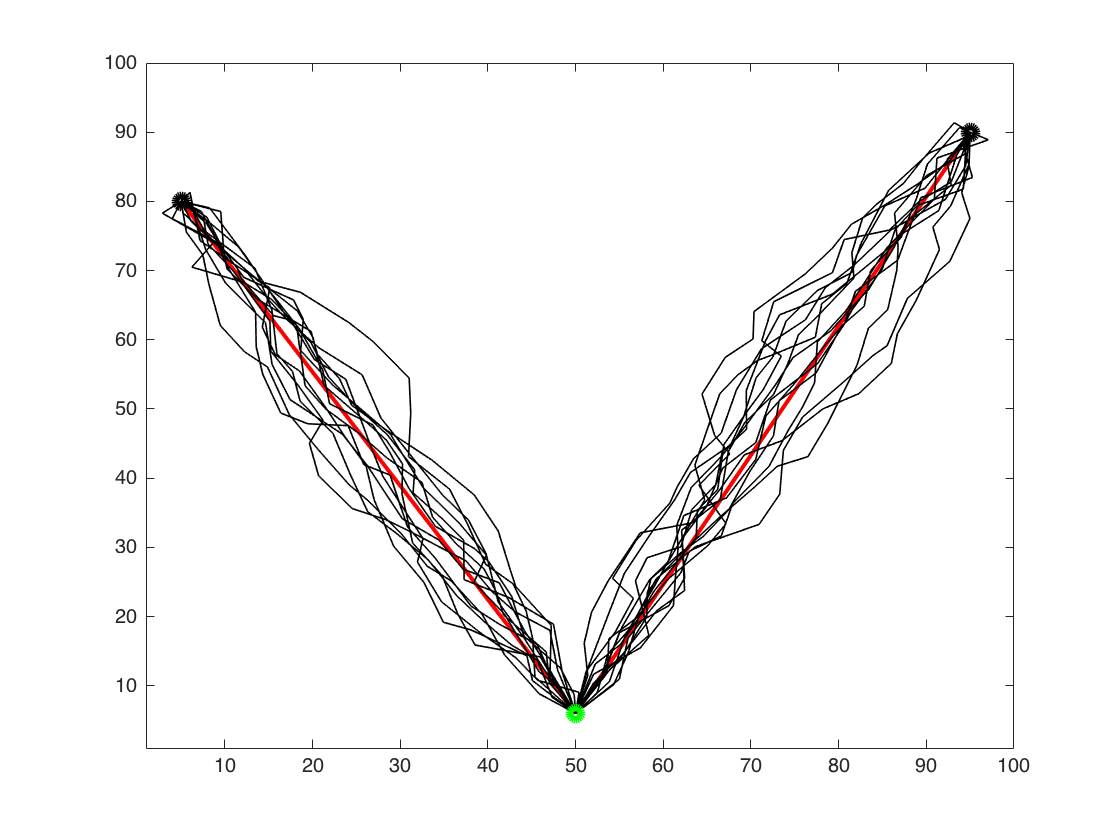
\includegraphics[width=0.8\linewidth]{figures/brownian_motion_mc.png}
	\caption{Brownian non-deterministic walks (black) surrounding deterministic cords (red). The starting point is indicated in green. For a set of $N=2$ possible trajectories, $15$ random walks around each trajectory with a variance of $10$. All distance units in meters.}
\end{figure}

\subsection{Selecting An Optimal Monte Carlo Trajectory} \label{sec:mcselbesttraj}
In Section \ref{sec:mctrajsets}, a set of possible trajectories, $T$ was defined. The trajectory that is ultimately chosen by the introduced path finder is the path that minimizes the average uncertainty of the predicted target field, i.e. maximizes the loss function, $L(T)$.
Let $\hat{Z}(S)$ be a Kriging predicted field from a set of samples at known locations. Furthermore, let $\hat{Z}(S+\hat{T}_k)$ be the a Kriging predicted field from the set $S$ concatenated with a virtual set of samples $\hat{T}_k$. The values in the set $\hat{T}_k$ have not necessarily been sampled, but they contain, as samples, the previously predicted values, $\hat{Z}(T_k)$, at the known locations in $T_k$.

\begin{equation}
	samples(\hat{T}_k) = \hat{Z}(T_k)
\end{equation}

The variance of the field with real and virtual samples, $\text{var}\{\hat{Z}(S+\hat{T}_k)\}$, can then be calculated. Using the definition for $\Sigma_{\text{var}}(\cdot)$ from Section \ref{eq:fielduncert}, the path chosen is the trajectory that satisfies:

\begin{equation}
	\label{eq:mcfoundpath}
	P = \argmin_{T_k}\ \Sigma_{\text{var}}(\text{var}\{\hat{Z}(S+\hat{T}_k)\})
\end{equation}

\subsection{Monte Carlo Path Planning Algorithm}
The exploration algorithm initializes by directing the vehicle to sweep across the forward diagonal of the target field to collect an initial set of samples. An initial variogram is fit, and a Kriging prediction of the field is then made. The variances of all points on the target field are then calculated. The set, $S_{v}$, of points with the $N$ highest prediction variances are found (Section \ref{sec:highestvars}). A set of trajectories, $T$, is then calculated (Section \ref{sec:mctrajsets}). The trajectory that is predicted to minimize the total uncertainty of the target field is chosen as the next path of the exploration vehicle (Section \ref{sec:mcselbesttraj}). Once the vehicle completes the last path chosen, the field values and variances are predicted and calculated again. A new path is chosen in the same fashion. The algorithm terminates when it can no longer choose a path that can be accomplished with the amount of fuel that remains within the exploration vehicle. Another case of planner termination occurs When the average prediction variance of the field is zero, which ideally occurs when all locations have been sampled.

An algorithm for Kriging Monte Carlo Path Planning (Kriging MCPP) for a target field, $Z$, of size ($h\times w$) is introduced in Algorithm \ref{alg:mcpp}. The initial location of the vehicle is set to $\vect{s}_{c} = [0\ 0]^T$. The vehicle starts the path planner with $F$ units of fuel.

\begin{algorithm}[h!]
\caption{Monte Carlo Path Planning (MCPP) with The Kriging Method}\label{alg:mcpp}
\begin{algorithmic}[1]
\Procedure{Kriging\_MCPP}{$Z$}
	\BState \emph{Conduct Initial Sweep}:
	\State SetWaypoint($[h\ w]^T$)
	\BState \emph{Krig The Field}:
	\State $\hat{Z}, \text{var}\{\hat{Z}\}$ = KrigingPredictField($Z$, $S$)

	\BState \textbf{while} $F > 0$ \textbf{and} $\Sigma_{\text{var}} > 0$:
	\State $P = []$
	\State $\Sigma_{\text{min}} = \infty$ \\

	\BState \ \ \ \ \emph{Find the highest field variances}:
	\State \ \ \ \ \textbf{for}\ $k = 1 \text{:} N$
	\State \ \ \ \  \ \ \ \ $S_{v}(k) = \argmax_{\vect{s}} \ \text{var}\{\hat{Z}_{k}(\vect{s})\}$
	\State \ \ \ \ \ \ \ \ $\text{var}\{\hat{Z}_{k+1}(\vect{s})\} = \text{var}\{\hat{Z}_{k}(\vect{s})\} - S_{v}(k)$\\

	\BState \ \ \ \  \emph{Calculate trajectories to all points found}:
	\State \ \ \ \  $\forall s_k \in S_{v}(k)$:
	\State \ \ \ \  \ \ \ \ $s_d = s_k$
	\State \ \ \ \  \ \ \ \ $f = \Big\lceil \frac{\|\vect{s}_c - \vect{s}_d\|_2}{\alpha} \Big\rceil$
	\State \ \ \ \  \ \ \ \ $T(1) = \begin{bmatrix} s_{c_x} \\ s_{c_y} \\ \text{arctan2}(s_{d_y} - s_{c_y}, s_{d_x} - s_{c_x}) \end{bmatrix}$
	\State \ \ \ \  \ \ \ \ $\forall i \in (1, f - 1)$:
	\State \ \ \ \  \ \ \ \  \ \ \ \ $T(i+1) = T(i) + \begin{bmatrix} \alpha \cos \theta(i) \\ \alpha \sin \theta(i) \\ \text{atan2}(s_{d_y} - T(i)_y, s_{d_x} - T(i)_x) \end{bmatrix} + \begin{bmatrix} \vect{w}(i) \\ 0 \end{bmatrix}$
	\State \ \ \ \  \ \ \ \ $T(f) = \begin{bmatrix} s_{d_x} \\ s_{d_y} \\ \theta_{f-1} \end{bmatrix}$\\

	\BState \ \ \ \  \ \ \ \  \emph{Calculate estimated field confidence for trajectory computed}:
	\State \ \ \ \  \ \ \ \  $\forall i \in [1, f]$:
	\State \ \ \ \  \ \ \ \  \ \ \ \ $\text{samples}(\hat{S}_T)$ += $\hat{Z}(T(i))$
	\State \ \ \ \  \ \ \ \  \ \ \ \ $\text{locations}(\hat{S}_T)$ += $T(i)$
	\State \ \ \ \  \ \ \ \  \ \ \ \ $\hat{Z}_T, \text{var}\{\hat{Z}\}_T$ = KrigingPredictField($Z$, $\hat{S}_T$)
	\State \ \ \ \  \ \ \ \  \ \ \ \ $\Sigma_{\text{var}}(T) = \text{avg}(\text{var}\{\hat{Z}\}_T)$\\

	\State \ \ \ \  \ \ \ \  \ \ \ \ \textbf{if} $\Sigma_{\text{var}}(T) < \Sigma_{\text{min}}$ \textbf{and} \text{length($T$)} $< F$:
	\State \ \ \ \  \ \ \ \  \ \ \ \ \ \ \ \ $\Sigma_{\text{min}} = \Sigma_{\text{var}}(T)$
	\State \ \ \ \  \ \ \ \  \ \ \ \ \ \ \ \ $P = T$\\

	\BState \ \ \ \  \emph{Navigate through the chosen path}:
	\State \ \ \ \  $\forall p \in P$:
	\State \ \ \ \  \ \ \ \ SetWaypoint($p$) 
\EndProcedure
\end{algorithmic}
\end{algorithm}

In Algorithm \ref{alg:mcpp}, the function \texttt{SetWaypoint()} is an abstracted function which steers the vehicle in the direction of the waypoint specified, and blocks the code instruction until the waypoint has been met. The function \texttt{length(}$T$\texttt{)} finds the arc length of the path by connecting all points in the trajectory, $T$. For a deterministically calculated trajectory, $T$, the arc length is $\alpha |T|$.

\begin{figure}[hb!]
	\centering
	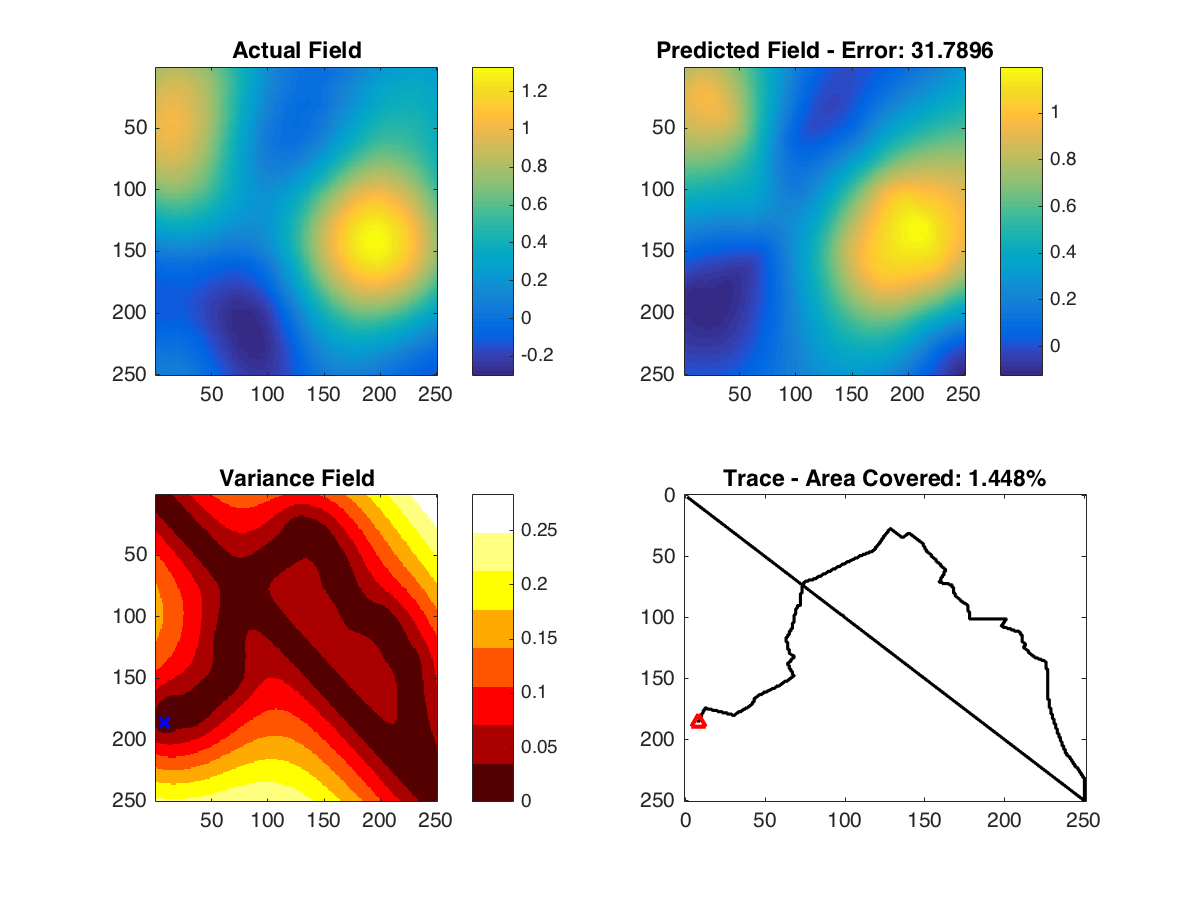
\includegraphics[width=0.95\linewidth]{figures/mc_4panel.png}
    \captionsetup{skip=0.20\baselineskip,size=footnotesize}
	\caption{The Next Highest Variance (NHV) algorithm (Section \ref{sec:nvh_pp_alg} terminated after two iterations of the algorithm. The actual field that is being explored is shown in the upper left. The current prediction of the actual field is shown in the upper right. The variance of the current prediction of the field is shown in the lower left. The trace of the exploration vehicle's path taken to the point of termination (in red) is shown in the lower right panel. All distance units are in meters. Here, $N$, the number of endpoints selected is $3$, and the number of random paths per cord calculated is $15$.}
	\label{fig:mcpp}
\end{figure}

\subsection{$N$ Next Highest Variances Algorithm (Zero Variance MCPP)} \label{sec:nnhv}
A small modification to the NHV algorithm can be made to consider more trajectories. If the set of highest variances on the field, $S_v$ has a cardinality greater than $1$ ($N > 1$), $N$ trajectories can be made, and weighed against each other in terms of their return on investment (as discussed in Section \ref{sec:mctrajsets}). This is done by selecting a zero variance gain on the noise of each Monte Carlo Path, and only calculating a single cord per endpoint. By weighing $N$ Next Highest Variances (N-NHV) against one another, more methodical routes can be taken. It may not always be the case that simply exploring the next highest variance will yield a smaller field variance. If a smaller prediction variance location is selected as the endpoint location (i.e. an endpoint that is not necessarily the first coordinate in the set $S_v$), the vehicle might sample more unknown points along the way, versus potentially rescanning already sampled area with the simple NHV algorithm.

\subsection{Benefits in MCPP over NHV}
The Monte Carlo based path planner takes into account a set of trajectories, and compares their estimated return on investment. The NHV simply takes the path to the high prediction uncertainty location. Though the MCPP algorithm, with a non-zero noise variance, does not deterministically calculate its trajectories, given enough trajectories, the algorithm could find a path that will reduce overall field uncertainty in a more methodical way over the NHV algorithm.

\subsection{Disadvantages of The Monte Carlo Path Planner}
The MCPP algorithm does not calculate the cost of each next move taken, but rather a set of waypoints taken. In other words, the algorithm only takes into account entire trajectories at a time. A more optimal approach to this planner would be to take into consideration the cost of each waypoint selected. A remedy to this problem using the MCPP would be to increase the number of random trajectories calculated for each cord.
